% =====================================================================
\section{Vector Fields}\label{ch:fields}
% =====================================================================

A \emph{vector field} is a function whose domain is a set of points in $\R^2$
(or $\R^3$) and whose range is a set of vectors in $\R^2$ (or $\R^3$) (Slides).
Think of the wind: at every point of a map there is a wind velocity, a vector
with a direction and a strength.

\subsection{Definitions}

\begin{definition}[Vector field on $\R^2$; Slides, Definition 1]\label{def:vf2}
Let $D$ be a set in $\R^2$ (a plane region). A \emph{vector field on $\R^2$} is a
function $\vF$ that assigns to each point $(x,y)$ in $D$ a two-dimensional
vector $\vF(x,y)$:
\[
  \vF(x,y)=\ip{M(x,y),\,N(x,y)}=M(x,y)\,\vi+N(x,y)\,\vj .
\]
\end{definition}

\begin{definition}[Vector field on $\R^3$; Slides, Definition 2]\label{def:vf3}
Let $E$ be a set in $\R^3$ (a solid region). A \emph{vector field on $\R^3$} is a
function $\vF$ that assigns to each point $(x,y,z)$ in $E$ a three-dimensional
vector:
\[
  \vF(x,y,z)=\ip{M,\,N,\,P}=M(x,y,z)\,\vi+N(x,y,z)\,\vj+P(x,y,z)\,\vk .
\]
\end{definition}

The scalar functions $M,N$ (and $P$) are the \emph{component functions} of
$\vF$. $\vF$ is \emph{continuous} if and only if its components are continuous.
(Some books write $P,Q,R$ instead of $M,N,P$.)

\begin{remark}[Position vector notation; Slides]\label{rem:position}
We identify the point $(x,y)$ with its \emph{position vector}
$\vx=\ip{x,y}$, and write $\vF(\vx)$ instead of $\vF(x,y)$:
\[
  (x,y)\;\longmapsto\;\vx=\ip{x,y}\;\longmapsto\;\vF(\vx)=\vF(x,y).
\]
Similarly in three dimensions, $(x,y,z)\mapsto\vx=\ip{x,y,z}\mapsto\vF(\vx)$.
This notation lets one formula cover both dimensions; e.g.\ $\vF(\vx)=\vx$ is
the field whose arrow at each point is its own position vector.
\end{remark}

\subsection{Sketching a vector field}

\begin{strategy}{Strategy (sketching $\vF$ by hand).}
\begin{enumerate}
  \item Choose a few points $(x,y)$, often a small grid, and make a table of
        $\vF(x,y)$.
  \item At each point draw the arrow $\vF(x,y)$ \emph{starting at that point}
        (if the arrows are long, scale all of them by the same factor).
  \item Look for structure: Is $\vF\cdot\vx=0$ (arrows tangent to circles about
        the origin)? Is $\vF$ a multiple of $\vx$ (radial)? Where is $\vF=\vzero$?
        Where is a component zero (horizontal or vertical arrows)? How does
        $\norm{\vF}$ grow?
\end{enumerate}
\end{strategy}

\begin{example}[Slides, Example 7.1]\label{ex:7.1}
A vector field in $\R^2$ is defined by $\vF(x,y)=-y\,\vi+x\,\vj$. Describe $\vF$
by sketching some of the vectors $\vF(x,y)$.
\end{example}
\begin{solution}
\step{1}{Table of values.}
\begin{center}
\renewcommand{\arraystretch}{1.2}
\begin{tabular}{cc@{\qquad}cc@{\qquad}cc}
\toprule
$(x,y)$ & $\vF(x,y)$ & $(x,y)$ & $\vF(x,y)$ & $(x,y)$ & $\vF(x,y)$\\
\midrule
$(1,0)$ & $\ip{0,1}$ & $(2,2)$ & $\ip{-2,2}$ & $(3,0)$ & $\ip{0,3}$\\
$(0,1)$ & $\ip{-1,0}$ & $(-2,2)$ & $\ip{-2,-2}$ & $(0,3)$ & $\ip{-3,0}$\\
$(-1,0)$ & $\ip{0,-1}$ & $(-2,-2)$ & $\ip{2,-2}$ & $(-3,0)$ & $\ip{0,-3}$\\
$(0,-1)$ & $\ip{1,0}$ & $(2,-2)$ & $\ip{2,2}$ & $(0,-3)$ & $\ip{3,0}$\\
\bottomrule
\end{tabular}
\end{center}
\step{2}{Structure.} With $\vx=\ip{x,y}$,
\[
  \vx\cdot\vF(\vx)=x(-y)+y(x)=0,
\]
so each arrow is perpendicular to the position vector, hence \emph{tangent to the
circle centred at the origin} through that point. Moreover
\[
  \norm{\vF(x,y)}=\sqrt{(-y)^2+x^2}=\sqrt{x^2+y^2}=r,
\]
so the arrows get longer in proportion to the distance from the origin. At
$(1,0)$ the arrow is $\ip{0,1}$ (upward), so the circulation is
\emph{counterclockwise}.

\textbf{Conclusion.} $\vF$ looks like the velocity field of a wheel rotating
counterclockwise about the origin (Figure~\ref{fig:rotation}); this is the
field of Figure~6 on the slides.
\end{solution}

\begin{figure}[H]
  \centering
  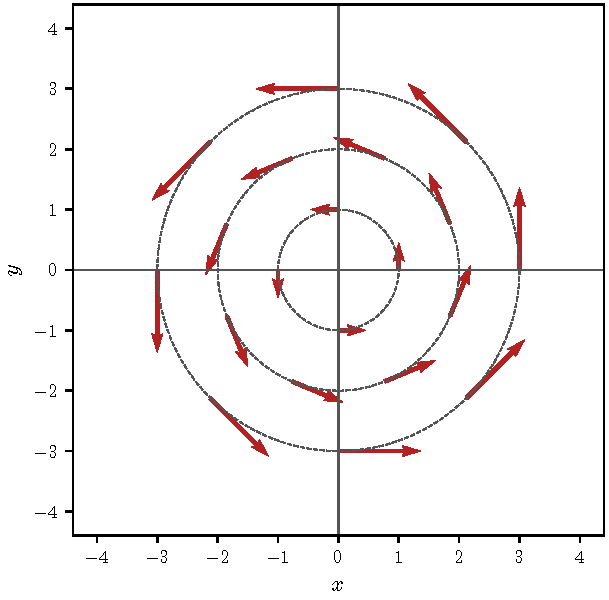
\includegraphics[width=0.48\linewidth]{rotation_field}
  \caption{$\vF(x,y)=\ip{-y,x}$ (arrows scaled by $\frac{1}{2.2}$). Each arrow is
  tangent to the dashed circle through its base point, with length equal to the
  radius.}
  \label{fig:rotation}
\end{figure}

\begin{exercise}[Slides, Exercise 1]\label{ex:exercise1}
Sketch the vector field $\vF(x,y)=y\,\vi+\frac12(y-x)\,\vj$ by drawing its vectors at
the nine points $(x,y)$ with $x,y\in\{-1,0,1\}$.
\end{exercise}
\begin{solution}
\step{1}{Compute.} $\vF(x,y)=\ip{y,\;\frac{y-x}{2}}$:
\begin{center}
\renewcommand{\arraystretch}{1.2}
\begin{tabular}{c|ccc}
\toprule
 & $x=-1$ & $x=0$ & $x=1$\\
\midrule
$y=1$ & $\ip{1,1}$ & $\ip{1,\frac12}$ & $\ip{1,0}$\\
$y=0$ & $\ip{0,\frac12}$ & $\ip{0,0}$ & $\ip{0,-\frac12}$\\
$y=-1$ & $\ip{-1,0}$ & $\ip{-1,-\frac12}$ & $\ip{-1,-1}$\\
\bottomrule
\end{tabular}
\end{center}
For instance at $(-1,1)$: $\ip{1,\frac{1-(-1)}{2}}=\ip{1,1}$; at $(1,0)$:
$\ip{0,\frac{0-1}{2}}=\ip{0,-\frac12}$.
\step{2}{Draw.} Attach each arrow to its point (Figure~\ref{fig:exercise1}).
The field vanishes at the origin; above the $x$-axis the arrows point right,
below they point left, and on the $x$-axis they are vertical. The overall
pattern is a clockwise swirl around the origin. (Compare with the GeoGebra
answer linked on the slide.)
\end{solution}

\begin{figure}[H]
  \centering
  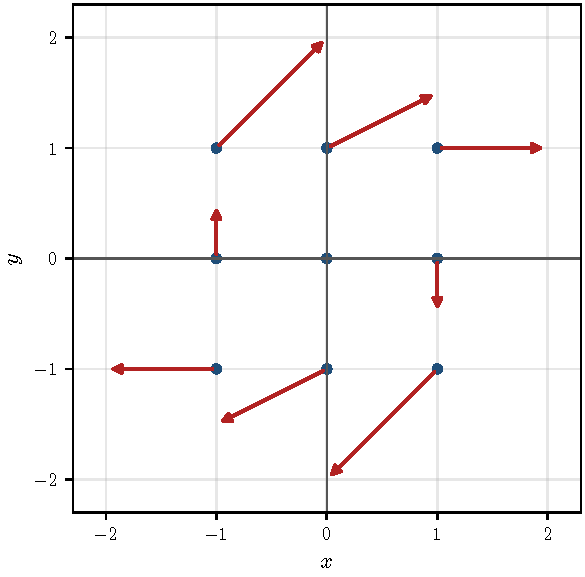
\includegraphics[width=0.46\linewidth]{exercise1}
  \caption{Exercise 1: $\vF=y\,\vi+\frac12(y-x)\,\vj$ at the nine indicated
  points (true length, no scaling).}
  \label{fig:exercise1}
\end{figure}

\begin{exercise}[Slides, Exercise 2]\label{ex:exercise2}
Match each vector field with its plot on the slide (four coloured panels):
\[
\text{A. }\vF=\ip{-\tfrac12,\tfrac12}\quad
\text{B. }\vF=\ip{\tfrac x2,\tfrac y2}\quad
\text{C. }\vF=\ip{1,\sin y}\quad
\text{D. }\vF=-\frac{\ip{x,y}}{\sqrt{x^2+y^2}} .
\]
\end{exercise}
\begin{solution}
Identify one distinguishing feature of each field first.
\begin{itemize}
\item \textbf{A} is \emph{constant}: every arrow is the same vector, pointing up and
      to the left at $135^\circ$. $\Rightarrow$ the \textbf{blue} panel (top right),
      where all arrows are identical and parallel.
\item \textbf{B} $=\frac12\vx$ is \emph{radial outward} with length $\frac12r$, so the
      arrows grow as we move away from the origin. $\Rightarrow$ the
      \textbf{orange} panel (bottom left).
\item \textbf{C} has $x$-component always $1$, so every arrow points to the right.
      Its $y$-component $\sin y$ is $0$ on the lines $y=0,\pm\pi$ (horizontal arrows),
      positive for $0<y<\pi$ and negative for $-\pi<y<0$; the arrows do not
      depend on $x$. $\Rightarrow$ the \textbf{yellow} panel (bottom right), whose
      rows of arrows are identical across each horizontal line.
\item \textbf{D} $=-\vx/\norm{\vx}$ has length $1$ everywhere and points
      \emph{toward the origin}. $\Rightarrow$ the \textbf{green} panel (top left),
      radial with arrows of equal length.
\end{itemize}
Answer: A--blue, B--orange, C--yellow, D--green
(Figure~\ref{fig:exercise2} redraws each field with its formula).
\end{solution}

\begin{figure}[H]
  \centering
  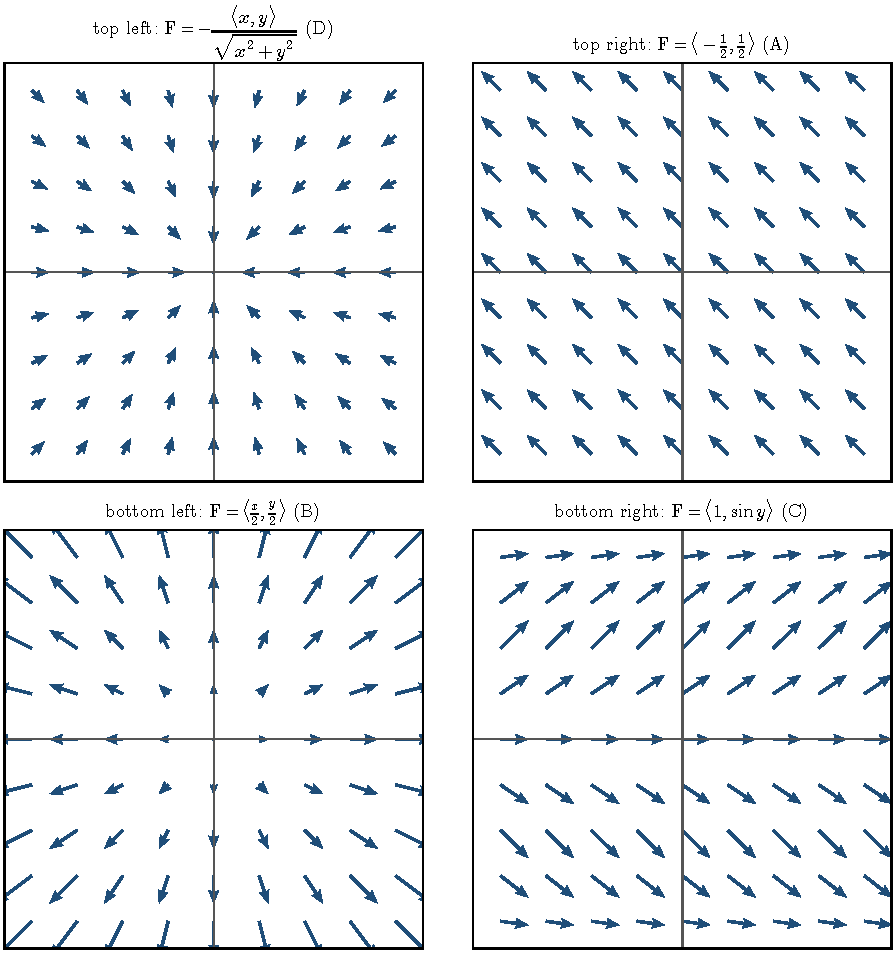
\includegraphics[width=0.78\linewidth]{exercise2}
  \caption{Exercise 2 redrawn: each panel is in the position of the
  corresponding coloured panel on the slide, labelled with its field.}
  \label{fig:exercise2}
\end{figure}

\begin{exercise}[Slides, Exercise 3]\label{ex:exercise3}
Which vector field has the plot shown on the slide (arrows in space, all
pointing upward and fanning outward away from the $z$-axis)?\\
A. $\vF=\ip{1,2,3}$\quad B. $\vF=\ip{1,2,z}$\quad C. $\vF=\ip{x,y,3}$\quad D. $\vF=\ip{x,y,z}$
\end{exercise}
\begin{solution}
\begin{itemize}
\item A is constant: all arrows would be parallel. The plot's arrows spread
      out, so not A.
\item B and D have $\vk$-component $z$, which is negative below the
      $xy$-plane, so some arrows would point \emph{down}; in the plot every arrow
      points up. Not B, not D. (D would be radial from the origin.)
\item C: the $\vk$-component is the constant $3>0$ (always up, same vertical
      size), while the horizontal part $\ip{x,y}$ points away from the $z$-axis
      and grows with the distance from it: exactly the fanning pattern.
\end{itemize}
Answer: \textbf{C}, $\vF(x,y,z)=\ip{x,y,3}$ (Figure~\ref{fig:exercise3}).
(On the slide, B--D are written as ``$\vF(x,y)$''; since they involve $z$ they
should read $\vF(x,y,z)$.)
\end{solution}

\begin{figure}[H]
  \centering
  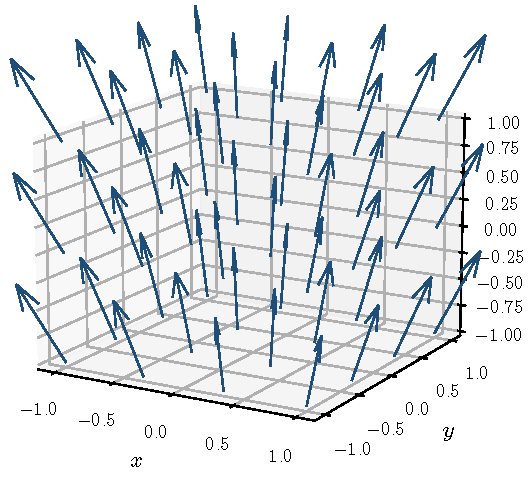
\includegraphics[width=0.5\linewidth]{exercise3}
  \caption{Exercise 3: $\vF(x,y,z)=\ip{x,y,3}$.}
  \label{fig:exercise3}
\end{figure}

\subsection{Computer-generated vector fields}

For anything but the simplest fields we let a computer draw the arrows,
usually scaled so they do not overlap. Figure~\ref{fig:computer} reproduces the
three examples on the slides. Notice how the formula is visible in the picture:
in $\ip{y,\sin x}$ the arrows are horizontal along the lines $x=k\pi$ (where
$\sin x=0$), and in $\ip{\ln(1+y^2),\ln(1+x^2)}$ both components are $\ge0$, so
every arrow points into the first-quadrant directions (right and/or up).

\begin{figure}[H]
  \centering
  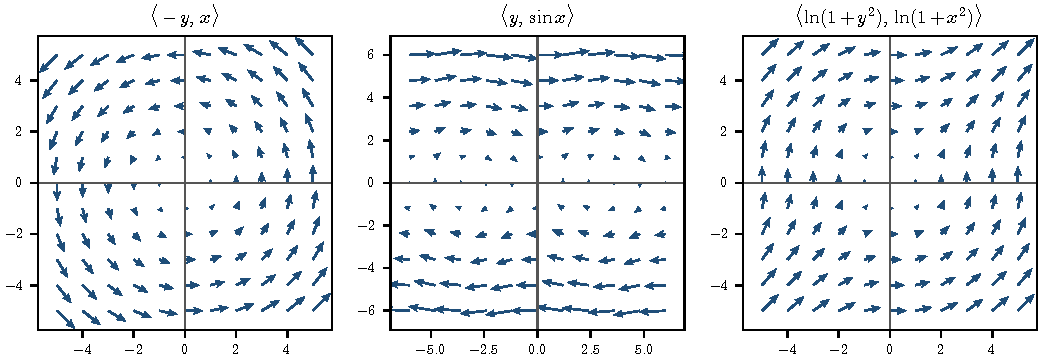
\includegraphics[width=\linewidth]{computer_fields}
  \caption{Slides, Figures 6--8: $\ip{-y,x}$, $\ip{y,\sin x}$ and
  $\ip{\ln(1+y^2),\ln(1+x^2)}$.}
  \label{fig:computer}
\end{figure}

\interactive{https://www.desmos.com/calculator/cho2h9ztfa}{Open the slide's Desmos graph}
(a gradient field drawn as arrows on a grid; see Example~\ref{ex:7.2}); edit
the two components to draw any other planar field. Appendix~\ref{app:interactive}
explains how to do the same in Python.

\subsection{Fields in physics}

\textbf{Velocity fields} (Slides, \emph{Application}). Wind patterns, ocean
currents and the airflow past an airfoil are described by assigning to each
point the velocity of the fluid there; the arrows on the slide's San Francisco
Bay and Nova Scotia maps are exactly such vectors.

\begin{example}[Gravitational field]\label{ex:gravity}
By Newton's law of gravitation, a mass $M$ at the origin attracts a mass $m$
at $\vx=\ip{x,y,z}$ with a force of magnitude $\dfrac{mMG}{\norm{\vx}^2}$ directed
toward the origin. Write the force as a vector field.
\end{example}
\begin{solution}
The unit vector from $\vx$ toward the origin is $-\vx/\norm{\vx}$. Multiplying by
the magnitude,
\[
  \vF(\vx)=-\frac{mMG}{\norm{\vx}^2}\cdot\frac{\vx}{\norm{\vx}}=-\frac{mMG}{\norm{\vx}^3}\,\vx
  =\ip{\frac{-mMGx}{(x^2+y^2+z^2)^{3/2}},\frac{-mMGy}{(x^2+y^2+z^2)^{3/2}},\frac{-mMGz}{(x^2+y^2+z^2)^{3/2}}}.
\]
All arrows point toward the origin and shrink like $1/r^2$
(Figure~\ref{fig:gravity}). The \emph{electric} force exerted by a charge $Q$ at
the origin on a charge $q$ at $\vx$, $\vF=\dfrac{\varepsilon qQ}{\norm{\vx}^3}\vx$
(Coulomb's law), has the same shape, pointing away from the origin when
$qQ>0$.
\end{solution}

\begin{figure}[H]
  \centering
  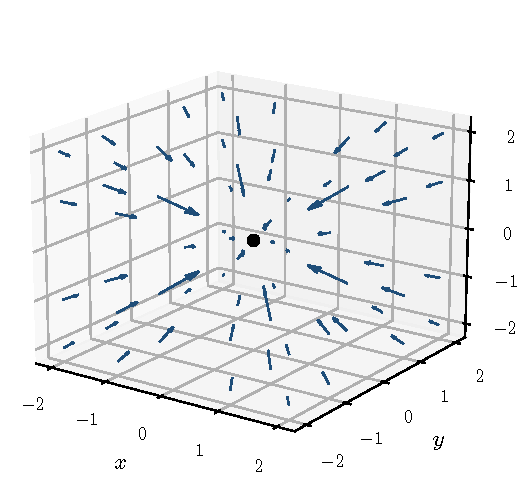
\includegraphics[width=0.48\linewidth]{gravity_field}
  \caption{An inverse-square field $\vF=-\vx/\norm{\vx}^3$: arrows point toward
  the origin and are much longer nearby.}
  \label{fig:gravity}
\end{figure}

\begin{example}\label{ex:zk}
Describe the vector field $\vF(x,y,z)=z\,\vk$.
\end{example}
\begin{solution}
Every arrow is vertical. At height $z$ its length is $|z|$: arrows point up
above the $xy$-plane, down below it, and vanish on the $xy$-plane. All points
at the same height carry the same arrow, since $\vF$ does not depend on $x$ or
$y$.
\end{solution}
